\documentclass[a4paper]{article}
% Pacotes necessários
\usepackage[portuguese]{babel}
\usepackage[backend=biber, style=apa, citestyle=apa, language=portuguese]{biblatex}
\usepackage{csquotes}
\addbibresource{Recursos/referencias.bib}

\usepackage{amsmath}
\usepackage{graphicx}
\usepackage{subcaption}
\usepackage{setspace}
\usepackage{siunitx} % Required for alignment
\sisetup{
  round-mode          = places, % Rounds numbers
  round-precision     = 2, % to 2 places
}
\usepackage{enumerate}
\usepackage{enumitem}
\usepackage{amsmath}
\usepackage{karnaugh-map}
\usepackage[section]{placeins}
\usepackage{geometry}
\usepackage{amssymb}
\usepackage{titling}
\usepackage[T1]{fontenc}
\usepackage{float}
\usepackage[hidelinks]{hyperref}
\usepackage{xcolor}
\usepackage{indentfirst}
\usepackage{array}
\usepackage{soul}
\usepackage{afterpage}
\newcolumntype{P}[1]{>{\centering\arraybackslash}p{#1}}
\onehalfspacing


% Comando para criar uma página vazia
\newcommand\myemptypage{
    \null
    \thispagestyle{empty}
    \addtocounter{page}{-1}
    \newpage
}

% Página de título principal
\newcommand{\firsttitlepage}{
    \begin{titlepage}
        \centering
        \vspace*{1cm}
        
        % Logos superior
        \begin{figure}[h!]
            \centering
            
\includegraphics[width=6cm]{Recursos/LOGO_IPB} % Substitua pelo caminho da imagem
            \vspace{0.5cm}
        \end{figure}

        % Informações da instituição
        \large\textbf{INSTITUTO POLITÉCNICO DE BEJA} \\
        \large\textbf{Escola Superior de Tecnologia e Gestão} \\
        \large\textbf{Mestrado em Engenharia de Segurança Informática} \\
        \large\textbf{Linguagens de Programação Informática} \\
        
        \vspace{2cm}
        
        % Título do projeto
        {\Huge \textbf{Caso 1}} \\
        
        \vspace{1.5cm}
        
        % Autores
        \large Paulo António Tavares Abade - 23919 \\
        
        \vfill
        
        % Logo inferior
        \begin{figure}[h!]
            \centering
            
\includegraphics[width=6cm]{Recursos/IPBejaESTIG.jpg} % Substitua pelo caminho da imagem
        \end{figure}
        
        \vspace{1cm}
        
        % Local e data
        {\large Beja, outubro de 2025}
    \end{titlepage}
}

\newcommand{\secondtitlepage}{
    \begin{titlepage}
        \centering
        \vspace*{1cm}
        
        % Informações da instituição
        \large\textbf{INSTITUTO POLITÉCNICO DE BEJA} \\
        \large\textbf{Escola Superior de Tecnologia e Gestão} \\
        \large\textbf{Mestrado em Engenharia de Segurança Informática} \\
        \large\textbf{Linguagens de Programação Informática} \\
        
        \vspace{2cm}
        
        % Título do projeto
        {\Huge \textbf{Caso 1}} \\
        
        \vspace{1.5cm}
        
        % Autores
        \large Paulo António Tavares Abade - 23919 \\

        \vspace{2cm}

        % Orientador
        \large Orientador: Armando de Jesus Ventura \\
        
        \vfill
        
        % Local e data
        {\large Beja, outubro de 2025}
    \end{titlepage}
}

\begin{document}


\pagenumbering{gobble} % Oculta numeração da página

% Primeira página de título
\firsttitlepage

\secondtitlepage


% Abstract
\section*{\LARGE\textbf{\textit{Resumo}}}

Neste trabalho será apresentada a resolução do trabalho prático referente à parte Python, onde é pedida a criação de uma aplicação 
com menu em linha de comandos que permita ao utilizador: Fazer Port Scanning, fazer um DoS Attack a um endereço IPv4, fazer um Syn Flood Attack 
a um endereço IPv4, fazer um script que analise ficheiros de log de pelo menos dois serviços, fazer um script de troca de mensagens encriptadas 
entre um cliente e um servidor, fazer um cliente de Port Knocking e fazer um script de gestão de passwords. Tudo isto utilizando a linguagem Python e 
algumas das bibliotecas disponíveis para a mesma, em um ambiente virtual com o sistema operativo Kali Linux.


\vspace{1cm}
% Keywords
\textbf{Keywords:} PortScanning, DoS Attack, Syn Flood Attack, Análise de Logs, Mensagens Encriptadas, Port Knocking, Gestão de Passwords
\newpage
%--------------------------------------------------------------------------------------------------------------------------------------

\section*{\LARGE\textbf{\textit{Abstract}}}

This work will present the solution to the practical assignment related to the Python portion, which requires the creation of an application
with a command-line menu that allows the user to: Perform Port Scanning, perform a DoS attack on an IPv4 address, perform a Syn Flood attack
on an IPv4 address, create a script that analyzes log files from at least two services, create a script for exchanging encrypted messages
between a client and a server, create a Port Knocking client, and create a password management script. All of this using the Python language and
some of the available libraries, in a virtual environment with the Kali Linux operating system.



\vspace{1cm}
% Keywords
\textbf{Keywords:} PortScanning, DoS Attack, Syn Flood Attack, Log Analysis, Encrypted Messages, Port Knocking, Password Management
\renewcommand{\contentsname}{Índice}       % Título do sumário
\renewcommand{\listfigurename}{Índice de Figuras} % Título da lista de figuras

% Início do conteúdo do relatório
\newpage
\doublespacing
\tableofcontents
\listoffigures
\doublespacing

\newpage
\pagenumbering{arabic}

\section{Introdução}\label{introducao}
Neste trabalho será apresentada a resolução do trabalho prático referente à parte Python, onde é pedida a criação de uma aplicação 
com menu em linha de comandos que permita ao utilizador: Fazer Port Scanning, fazer um DoS Attack a um endereço IPv4, fazer um Syn Flood Attack 
a um endereço IPv4, fazer um script que analise ficheiros de log de pelo menos dois serviços, fazer um script de troca de mensagens encriptadas 
entre um cliente e um servidor, fazer um cliente de Port Knocking e fazer um script de gestão de passwords. Tudo isto foi realizado dentro de uma 
máquina virtual com o sistema operativo Kali Linux, utilizando a linguagem Python e algumas das bibliotecas disponíveis para a mesma. Foi 
testado em um ambiente controlado, onde havia permissão para realizar os ataques e análises necessárias.
\subsection{Análise dos Requisitos}
Para a realização deste trabalho prático, foi primeiro necessário compreender tudo o que estava a ser pedido para realizar o trabalho, 
sendo analisado nas próximas secções os temas mais teóricos que necessitaram de ser aprofundados para ser possível a sua implementação.
\subsubsection{Port Scanning}
O Port Scanning é uma técnica utilizada para identificar quais portas estão abertas, a escutar ou fechadas em um sistema de rede. Um exemplo 
de ferramenta popular para realizar Port Scanning é o Nmap (Network Mapper), como mostrado na Figura \ref{fig:nmap_port_scanning}. O Nmap pode 
ser utilizado para descobrir hosts e serviços em uma rede, criando um "mapa" da rede.
\begin{figure}
    \centering
    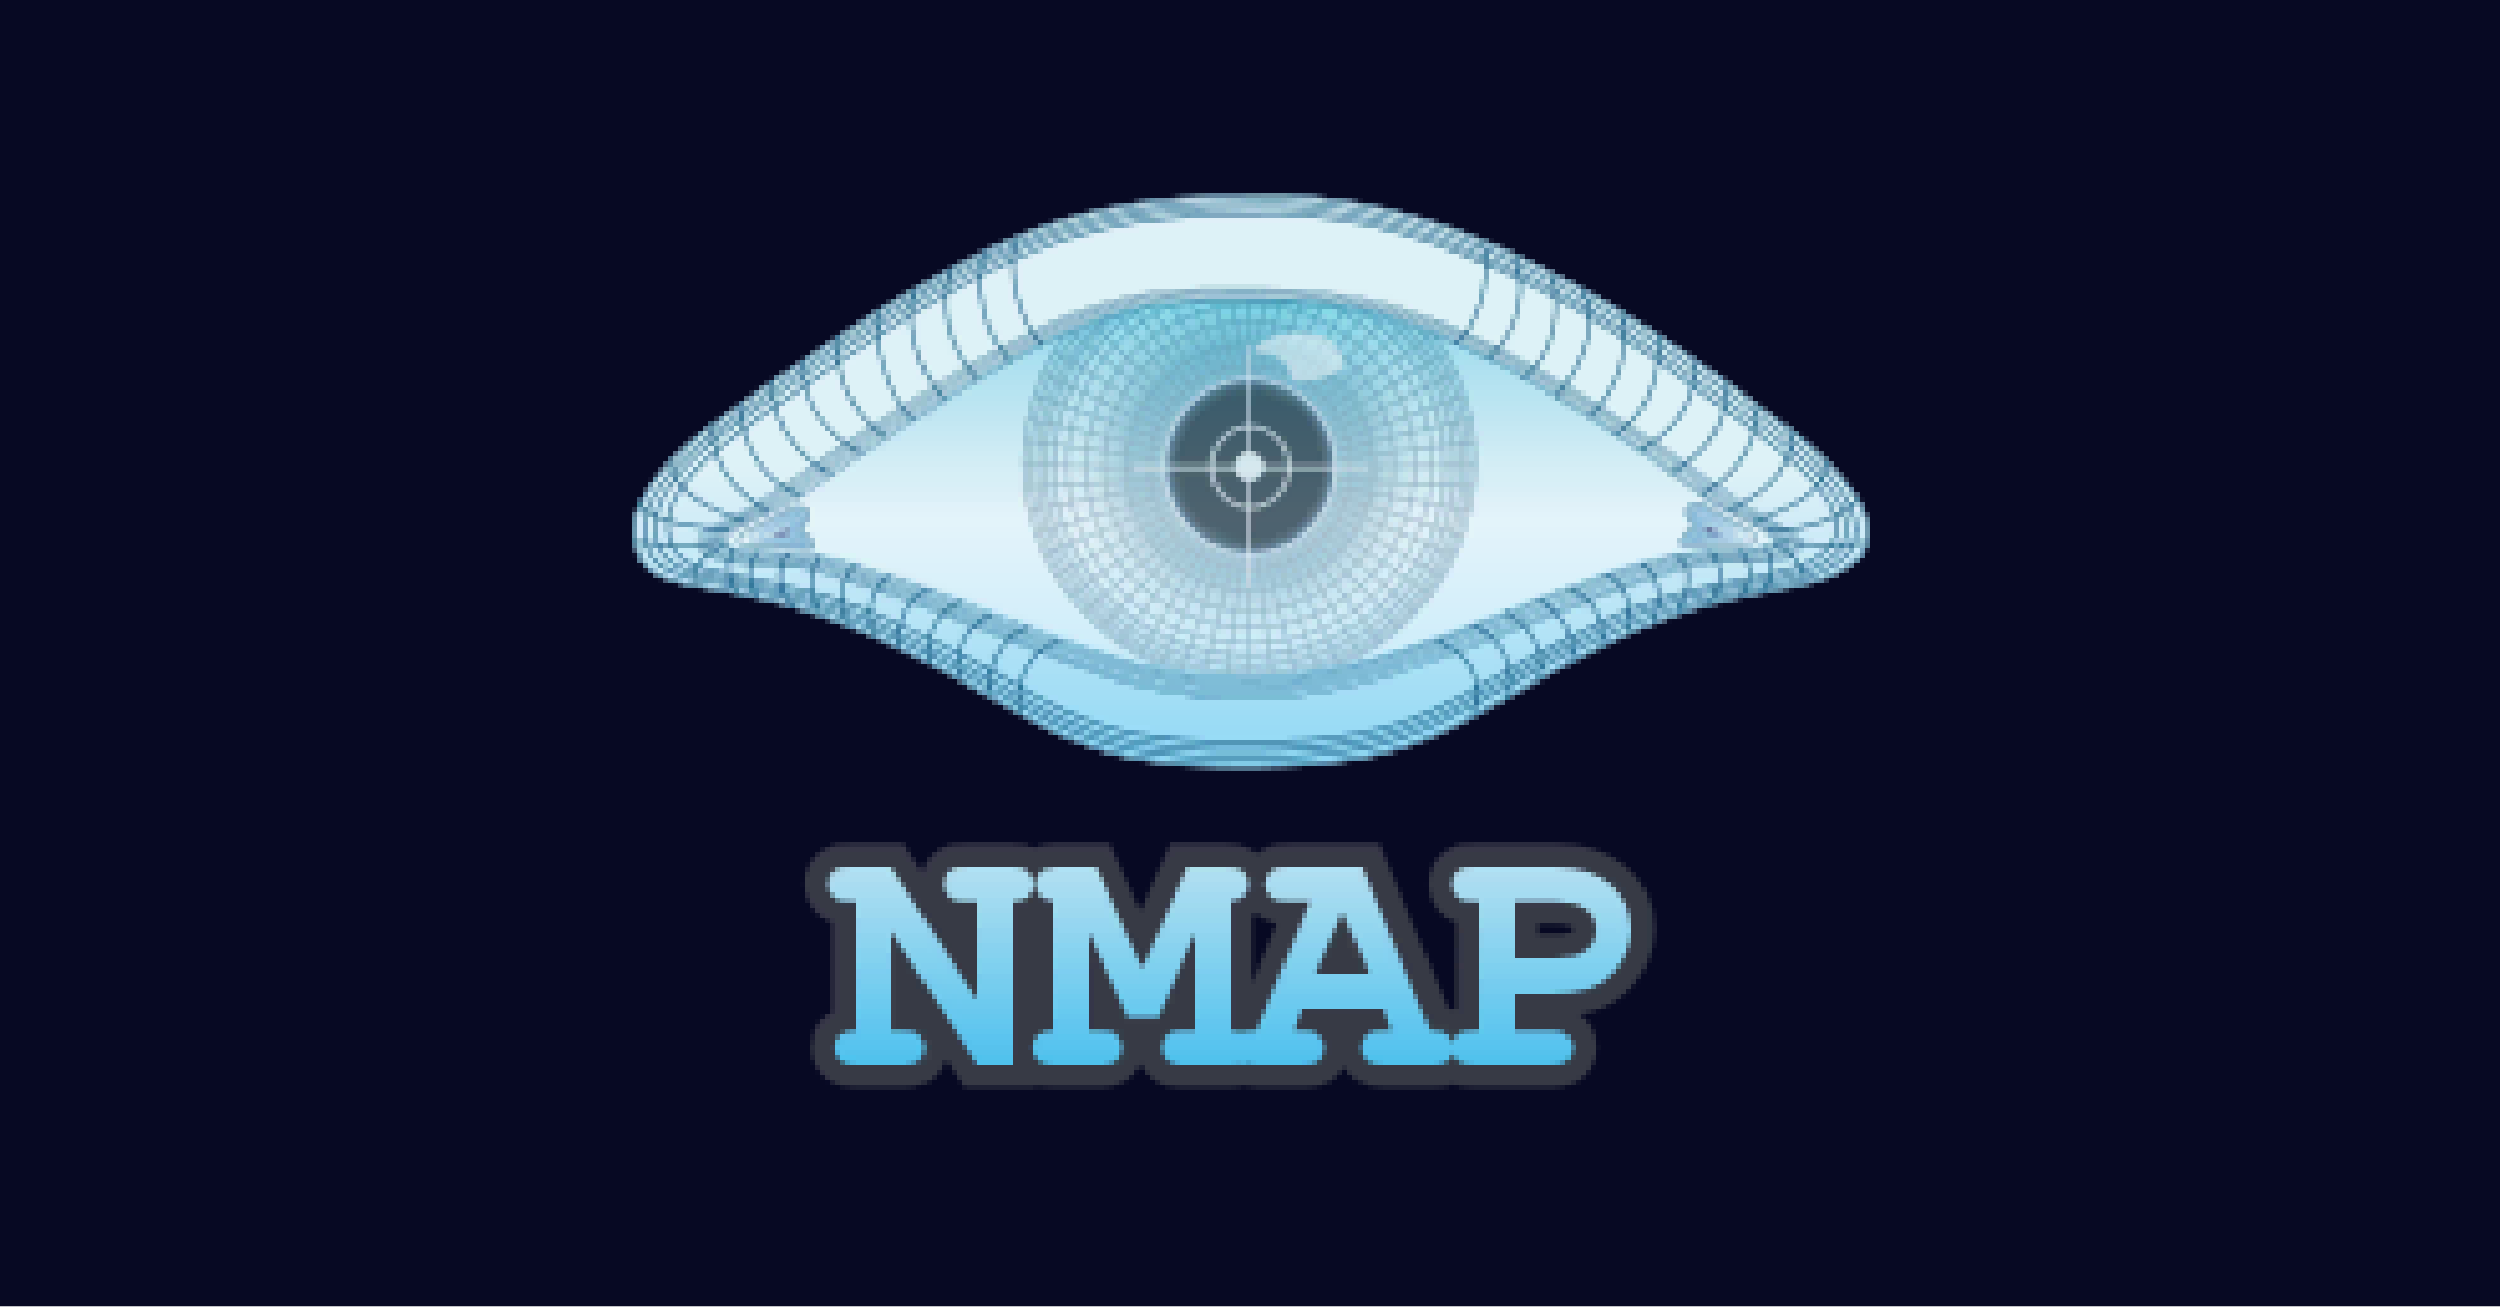
\includegraphics[width=0.7\textwidth]{Recursos/Nmap.png}
    \caption{Exemplo de Port Scanning com Nmap}
    \label{fig:nmap_port_scanning}
\end{figure}
\subsubsection{DoS Attack}
Um DoS (Denial of Service) Attack é um ataque que tem o objetivo de tornar um serviço indisponível para um ou mais utilizadores. Isso é 
feito através do envio de uma grande quantidade de tráfego para o alvo, através do protocolo UDP, já que este não espera uma resposta, o que facilita a
sobrecarga do sistema alvo. 
\subsubsection{Syn Flood Attack}
Um Syn Flood Attack é um tipo de ataque que explora o processo de handshake do protocolo TCP. O atacante envia uma grande quantidade de pacotes 
SYN para o alvo, mas nunca completa o handshake, o que leva o sistema a ficar sobrecarregado com conexões half-open. Isto pode resultar 
na indisponibilidade do serviço para os utilizadores.
\subsubsection{Port Knocking}
O Port Knocking é uma técnica de segurança que envolve o envio de uma sequência específica de pacotes para portas fechadas em um sistema. 
Quando a sequência correta é recebida, o sistema adiciona o endereço IP do remetente a uma lista de permissões temporária, permitindo o 
acesso ao dispositivo.
%---------------------------------------------------------------------------------------------------------------------------
\section{Desenvolvimento}\label{desenvolvimento}

Nesta secção será apresentado o desenvolvimento do trabalho prático, com a 
explicação de cada uma das funcionalidades implementadas.
\subsection{Port Scanner}
A funcionalidade de Port Scanning foi implementada utilizando a biblioteca \textit{\textbf{nmap}} 
do Python. Esta biblioteca permite a realização de varreduras de portas de forma simples e eficiente. O código pede 
ao utilizador um endereço IPv4, e em seguida pede um intervalo de portas a serem escaneadas. O resultado do escaneamento 
é apresentado ao utilizador, mostrando quais portas estão abertas, fechadas ou filtradas.
\subsection{DoS Attack}
A funcionalidade de DoS Attack foi implementada utilizando a biblioteca \textit{\textbf{scapy}} do Python. Esta biblioteca 
permite a criação e envio de pacotes de rede de forma flexível. O código pede ao utilizador um endereço IPv4 alvo, e em 
seguida pede a porta onde será feito o ataque. O código então envia uma grande quantidade de pacotes UDP para o alvo,
com o objetivo de sobrecarregar o sistema. O código foi feito a partir do exemplo apresentado no seguinte GitHub 
\url{https://github.com/M-Taghizadeh/PyDOS}, onde foi misturado com os contéudos de
\url{https://thepythoncode.com/article/syn-flooding-attack-using-scapy-in-python}. São utilizadas threads para enviar 
os pacotes de forma mais rápida. As bibliotecas utilizadas são: \textit{\textbf{scapy}}, \textit{\textbf{threading}} e 
\textit{\textbf{random}}.
\subsection{Syn Flood Attack}
A funcionalidade de Syn Flood Attack também foi implementada utilizando a biblioteca \textit{\textbf{scapy}} do Python.
O código pede ao utilizador um endereço IPv4 alvo, e em seguida pede a porta onde será feito o ataque. O código então
envia uma grande quantidade de pacotes SYN para o alvo, sem completar o handshake, com o objetivo de sobrecarregar o sistema.
O código foi feito a partir do exemplo apresentado no seguinte GitHub \url{https://thepythoncode.com/article/syn-flooding-attack-using-scapy-in-python}.
São utilizadas threads para enviar os pacotes de forma mais rápida. As bibliotecas utilizadas são: \textit{\textbf{scapy}} e \textit{\textbf{random}}.
\newpage

%---------------------------------------------------------------------------------------------------------------------------
\section{Conclusão}\label{conclusao}

%---------------------------------------------------------------------------------------------------------------------------

\newpage
\renewcommand{\refname}{Bibliografia} % Para artigos
\renewcommand{\bibname}{Bibliografia} % Para livros e relatórios
\addcontentsline{toc}{section}{Bibliografia} % Adiciona a Bibliografia ao índice
\printbibliography

\end{document}
